% set home directory
\providecommand{\homedir}{..} 
% load the preamble of main.tex by subfiles
\documentclass[\homedir/main.tex]{subfiles}
% ##############################################################################
\begin{document}

\setcounter{chapter}{0}
\chapter{序論}\label{sec:introduction}
\section{研究背景}
現代では,我々はしばしば色やエフェクトなどによって飾り付けられた文字を目にする.
このように装飾された文字は「デザイン文字」と呼ばれる.
デザイン文字は装飾のないシンプルな文字と比べ,目立ちやすく具体的なイメージを与えやすい点で優れている.
例えば,次の\cref{fig:design_char_ex}は赤い「炎」という文字に燃えているようなエフェクトを付与したものであるが,
装飾のない「炎」に比べメラメラと炎が燃えている印象が相手に良く伝わると考えられる.

\begin{figure}[ht]
    \centering
    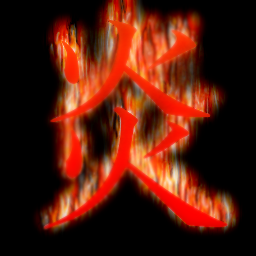
\includegraphics[keepaspectratio, scale=1.0]{design_character_example.png}
    \caption{デザイン文字の例}
    \label{fig:design_char_ex}
\end{figure}

デザイン文字は
目につくデザインは重要
デザインされた文字列は多くの分野で用いられている.
チラシ,ポスター,書籍の表紙,Webサイト,ロゴなど
そういったデザインを作成するのは,高度な技術や多大な時間を要することも多い.
スタイル転写の分野でCNNが成功を収めており,
デザイン作成支援への応用が研究されている.

\section{研究目的}
本研究の目的は,
文字列を含んだデザインの作成は技術や時間を要するが,
スタイル転写を応用することでこれを支援することを目的とする.
また、文字列を含んだデザインには歪みがあることがある.
こうした歪みは単にスタイルの転写を行うだけでは転写できない.
そこで、歪みのあるデザインからの歪みの推定・転写を可能にし、
単なるスタイル転写では扱えないものに対応することを目指す.

\section{本論文の構成}
本論文の構成は,次のようになっている.\\
第1章では,本研究の背景と目的について述べた.\\
第2章では,本研究に関連する先行研究について述べる.\\
第3章では,本研究の前提知識となる理論について述べる.\\
第4章では,実験内容とその結果について述べる.\\
第5章では,実験内容とその結果について述べる.\\
最後に第6章では,本論文の結論と今後の課題を述べる.

\printBibForSubfiles
\end{document}